\newpage
\vspace{2cm}
\begin{lstlisting}[language={[LaTeX]TeX}, label=liste, caption=Code d'un tableau basic, inputencoding=utf8/latin1, frame=single,numbers=left, numberstyle=\tiny]
\documentclass{report}
\begin{document}
			\begin{table}[h]
				\centering
          \begin{tabular}{| c | c |}
						\hline
						Tab & Tab\\
						\hline
					\end{tabular}
				\caption{Tableau basic}
				\label{tab:Tableau basic}
			\end{table}
\end{document}
\end{lstlisting}

\begin{multicols}{2}
		\blindtext[1]\\
\end{multicols}

\hspace*{-9mm}
\begin{minipage}[h]{115mm}
\begin{tabular}{| l | l |}
			\hline
			\multicolumn{2}{|>{\columncolor[gray]{0.9}}c|}{\bf \fontfamily{lmss}\selectfont Liste des packages latex}\\
			\hline
			\hline
			{\fontfamily{lmss}\selectfont \textbf{Utilit�}} & {\fontfamily{lmss}\selectfont \textbf{Les packages}}\\
			\hline
			\hline
			\hline
			Packages de langue & inputenc, fontenc, babel\\
			\hline
			Cr�ation d'un layout & layout\\
			\hline
			Modification des marges & geometry\\
			\hline
			Interligne & setspace\\
			\hline
			Soulignement & soul,ulem\\
			\hline
			Symbole \EUR & eurosym\\
			\hline
			Pack de police & bookman, charter, newcent\\
			\hline
			Citation d'url & url\\
			\hline
			Citation de code & verbatim, moreverb\\
			\hline
			Citation de code color� & listings\\
			\hline
			En-t�tes et pieds de pages personnalis�s & fancyhdr\\
      \hline
      \hline
\end{tabular}  
\end{minipage}
\begin{minipage}[h]{7cm}
%\fbox{encadr�}
%\shadowbox{ombr�}
%\ovalbox{entourn�}
%\doublebox{double encadr�}
%{\color{blue}\Ovalbox{\color{red}Hello}}
\ovalbox{ 
\begin{minipage}{6cm} 		
\renewcommand{\LettrineFontHook}{\color[gray]{0.5}}
\lettrine[lines=2]{L}{}orem ipsum dolor sit amet, consectetuer
adipiscing elit. Etiam lobortis
facilisis sem. Nullam nec mi et
neque pharetra sollicitudin. Praesent
imperdiet mi nec ante. Donec ullamcorper,
felis non sodales commodo, lectus
velit ultrices augue, a dignissim
nibh lectus placerat pede. Vivamus
nunc nunc, molestie ut, ultricies vel,
semper in, velit. Ut porttitor. Praesent
in sapien. Lorem ipsum dolor sitvelit 
ultrices augue, a dignissim
nibh lectus placerat pede. Vivamus
nunc nunc, molestie ut, ultricies vel,
semper in, velit. Ut porttitor. Praesent
in sapien. Lorem ipsum dolor sit\\
\end{minipage}
}
\end{minipage}

\boxput *(0 ,1){
\colorbox{white}{Titre de la boite}
}{
\setlength {\fboxsep }{6pt}
\fbox {\begin{minipage}{8cm}
Bla \\
Bla \\
Bla
\end{minipage}}
}

	\begin{center}
			\includegraphics[width=35mm]{linus}\\
	\bf \fontfamily{lmss}\selectfont  Linux, comme nous le savons tous, est grand... \\
	Il ex�cute une boucle infinie en \textcolor[rgb]{0.55,0,0}{5} secondes! \\\textcolor[rgb]{0.55,0,0}{Linus Benedict Torvalds, \tiny{1969}}\\
	\end{center}

\newpage
\JournalName{Freeways \& Moz}
\noindent\HorRule{3pt} \\[-0.75\baselineskip]
\HorRule{1pt}

\vspace*{2cm}
\begin{center}
\includegraphics[width =\textwidth , trim =0 0 0 0 , clip=true]{tmoz}
\end{center}

\vspace{0.5cm}
	\SepRule
\vspace{0.5cm}


\begin{tikzpicture}[remember picture,overlay]
\node[rotate=60,scale=14,text opacity=0.3]
  at (current page.center) {\textcolor[rgb]{0.55,0,0}{TOP SECRET}};
\end{tikzpicture}

\newpage
\begin{tikzpicture}[remember picture,overlay]
    \node[inner sep=0pt,opacity=0.1] at (current page.center) {%
        \includegraphics[width=\paperwidth,height=\paperheight]{1}%
    };%
\end{tikzpicture}

\fcolorbox{black}{green!70}{
\begin{minipage}{11cm}
\begin{center}
\Large \textbf{\textcolor{white}{\blindtext[1] }}
\end{center}
\end{minipage}}\\

\begin{enumerate}
\item a
\item a
\item a
\end{enumerate}

\begin{dinglist}{98}
\item a
\item a
\item a
\end{dinglist}

\newpage
\begin{tikzpicture}[remember picture,overlay]
    \node[inner sep=0pt] at (current page.center) {%
        \includegraphics[width=\paperwidth,height=\paperheight]{2}%
    };%
\end{tikzpicture}

% Now typeset a sample box.
\noindent 
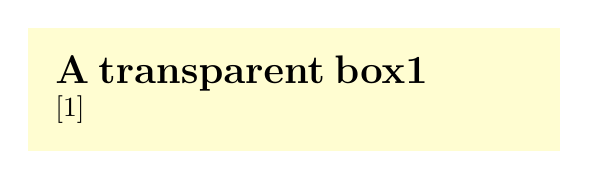
\begin{tikzpicture}
\node[text width=.5\textwidth,
      fill=yellow!30, 
      fill opacity=0.6,
      text opacity=1,
      inner sep=10pt]{
  {\bf\Large A transparent box1}\\
 \blindtext[1] 
};
\end{tikzpicture}\\
\vspace{2cm}
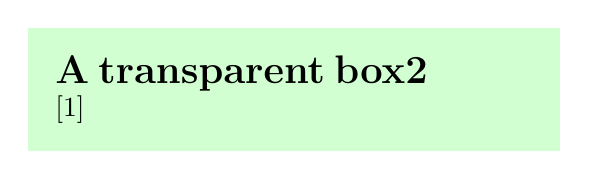
\begin{tikzpicture}
\node[text width=.5\textwidth,
      fill=green!30, 
      fill opacity=0.6,
      text opacity=1,
      inner sep=10pt]{
  {\bf\Large A transparent box2}\\
 \blindtext[1] 
};
\end{tikzpicture}